%% -*- mode: latex; mode: flyspell -*-
\documentclass[12pt, letter]{article}

%% Class name and Assignment number
%%
\newcommand{\courseName}{Introduction~to~Deep~Learning~for~Computer~Vision}
\newcommand{\assignName}{Assignment~6:~Debug a deep neural network}

%% Packages
\usepackage{amsmath,amsfonts,amssymb,amsthm,dsfont}
\usepackage{graphicx}
\usepackage[bookmarks=false]{hyperref}
\usepackage{color}
\usepackage{lipsum}

%% Paper format
\usepackage{geometry}
\geometry{
    letterpaper,
    %% total={216mm,279mm}, %< NSERC size
    margin=2.00cm,     %< default
    %% margin=1.87cm,       %< NSERC tightest
}

%% Headers and footers
\usepackage[explicit]{titlesec}
\newpagestyle{titlesec_assignment}{
  \sethead{\courseName}{}{\assignName}\setfoot{}{\thepage}{}
  \headrule
  %% \footrule
}

\begin{document}

%% Set header and footer
\pagestyle{titlesec_assignment}

%% Title
\title{\courseName\\\assignName}
\author{Kwang Moo Yi}
\maketitle

\abstract{This is an example abstract. \lipsum[1]}

\section{Example Section}

Example Section. \lipsum[1]

\subsection{Example Subsection}

Example Sub Section. \lipsum[1]

\paragraph{Example paragraph.} \lipsum[1]


\subsection{Example  Equation}

This is how a equation looks like.
\begin{equation}
  y = a x^2 + b x + c
  \;\;, 
\end{equation}
where an inline equation looks like $a=b$.

\subsection{Example  Figure}

To put a figure, you can do as shown in Fig.~\ref{fig:eg}.
%% 
\begin{figure}
  \centering
  \rule{2cm}{2cm} % Replace this with below, and your actual figure
  %% 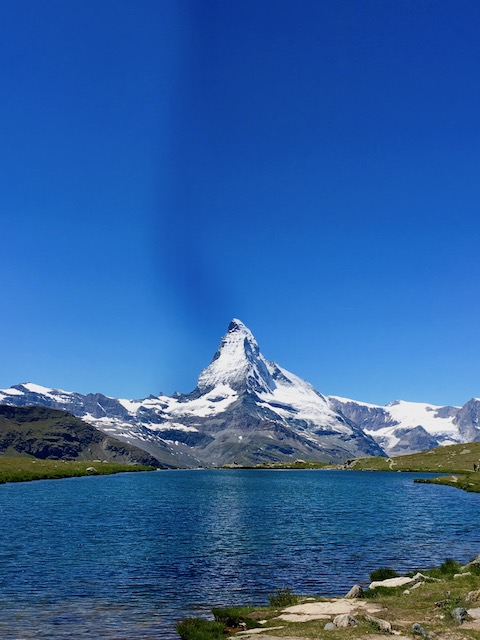
\includegraphics[width=0.4 \textwidth]{input.jpg}
  \caption{Example caption.}
  \label{fig:eg}
\end{figure}

\end{document}


%%% Local Variables:
%%% mode: latex
%%% TeX-master: t
%%% End:
